\newpage
\subsection{Caso d'uso UC7: Compilazione questionario}
\label{UC7}
\begin{figure}[h]
\centering
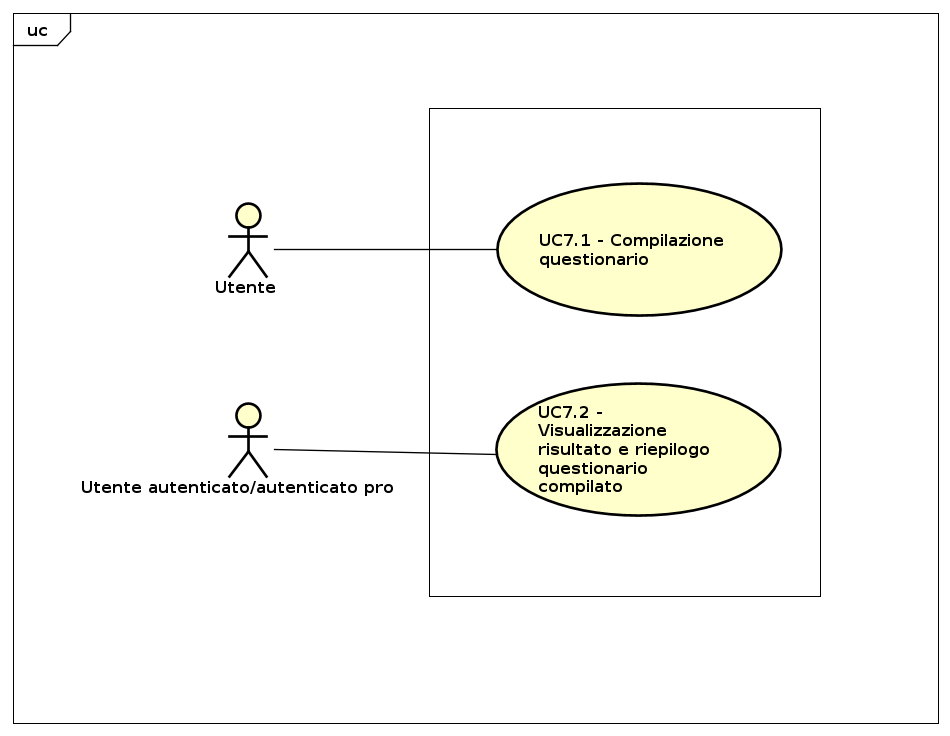
\includegraphics[scale=0.5,keepaspectratio]{UML/UC7.png}
\caption{UC7: Compilazione questionario}
\end{figure}
\FloatBarrier
\begin{itemize}
\item\textbf{Attori}: utente autenticato, utente autenticato pro;
\item\textbf{Descrizione}: l'attore che compila un questionario può rispondere alle domande che gli si presentano nell'ordine che preferisce spostandosi alla domanda successiva, a quella precedente oppure ad una a sua scelta e infine conferma le risposte date per poter visualizzare il risultato ottenuto e il riepilogo delle risposte date;
\item\textbf{Precondizione}: l'attore si è iscritto ad un questionario e l'autore del questionario ne ha abilitato la compilazione;
\item\textbf{Postcondizione}: l'attore visualizza la valutazione finale che ha ottenuto e il riepilogo delle risposte date;
\item\textbf{Scenario principale}:
\begin{itemize}
\item L'attore può passare alla domanda successiva (UC7.1);
\item L'attore può passare alla domanda precedente (UC7.2);
\item L'attore può passare ad una domanda a sua scelta (UC7.3);
\item L'attore può confermare le risposte date alle domande (UC7.4).
\end{itemize}
\item\textbf{Scenari alternativi}: nel caso in cui il questionario non è stato abilitato compare una schermata di attesa e l'attore può annullare l'operazione tornando alla schermata precedente.
\end{itemize}

\subsubsection{Caso d'uso UC7.1: Spostamento alla domanda successiva}
\label{UC7.1}
\begin{itemize}
\item\textbf{Attori}: utente autenticato, utente autenticato pro;
\item\textbf{Descrizione}: l'attore può passare alla domanda successiva;
\item\textbf{Precondizione}: l'attore sta compilando un questionario;
\item\textbf{Postcondizione}: il sistema visualizza la domanda successiva;
\item\textbf{Scenario principale}: l'attore seleziona il comando per passare alla domanda successiva.
\end{itemize}

\subsubsection{Caso d'uso UC7.2: Spostamento alla domanda precedente}
\label{UC7.2}
\begin{itemize}
\item\textbf{Attori}: utente autenticato, utente autenticato pro;
\item\textbf{Descrizione}: l'attore può passare alla domanda precedente;
\item\textbf{Precondizione}: l'attore sta compilando un questionario;
\item\textbf{Postcondizione}: il sistema visualizza la domanda precedente;
\item\textbf{Scenario principale}: l'attore seleziona il comando per passare alla domanda precedente.
\end{itemize}

\subsubsection{Caso d'uso UC7.3: Spostamento ad una domanda a scelta}
\label{UC7.3}
\begin{itemize}
\item\textbf{Attori}: utente autenticato, utente autenticato pro;
\item\textbf{Descrizione}: l'attore può passare ad una domanda a sua scelta selezionandola attraverso la tabella delle domande. Queste saranno identificate da un numero, in base all'ordine in cui sono poste all'interno del questionario, e da un colore, arancioni se è già stata data una risposta oppure grige in caso contrario;
\item\textbf{Precondizione}: l'attore sta compilando un questionario;
\item\textbf{Postcondizione}: il sistema visualizza la domanda selezionata dall'attore;
\item\textbf{Scenario principale}: l'attore seleziona una domanda a cui deve ancora rispondere o una alla quale vuole cambiare la risposta data.
\end{itemize}

\subsubsection{Caso d'uso UC7.4: Conferma risposte}
\label{UC7.4}
\begin{itemize}
\item\textbf{Attori}: utente autenticato, utente autenticato pro;
\item\textbf{Descrizione}: l'attore può confermare le domande a cui ha dato una risposta;
\item\textbf{Precondizione}: l'attore sta compilando un questionario;
\item\textbf{Postcondizione}: l'attore ha confermato le risposte date e il sistema visualizza una schermata contenente il riepilogo del questionario svolto e un voto;
\item\textbf{Scenario principale}: l'attore che ha finito di rispondere a tutte le domande conferma le risposte date;
\item\textbf{Scenari alternativi}: l'attore conferma le risposte date anche se non le ha compilate tutte, accettando il fatto che queste verranno considerate sbagliate.
\end{itemize}